
It is a priority that a user logs into the system for security reasons to be able to interact with it. When testing the login use case we tested for the user?s authentication and rights. We tested weather or not he has admin or normal user rights.

The local login page
\newline 
\newline 
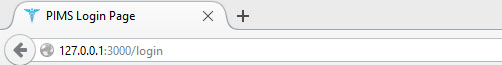
\includegraphics[width=200px]{./TestingDoc/Graphics/login}
\newline 
\newline 
Successfu.l login unit tests
\newline 
\newline 
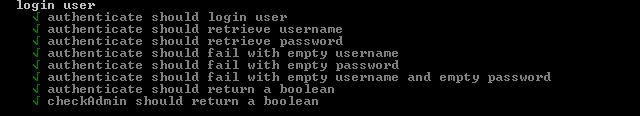
\includegraphics[width=350px]{./TestingDoc/Graphics/LoginTests}	
\subsubsection*{Conditions}
The following pre and post conditions are defined for adding a new user.
	
\subsubsection*{Pre conditions}	
\begin{itemize}
		\item User must not be logged in
		\item User must have valid credentials, a valid username and password.
		\item User credentials must be found in the Mongo database.
\end{itemize}	

\subsubsection*{Post conditions}	
\begin{itemize}
		\item User successfully logged in according to his user rights
\end{itemize}	

Code snippets for user login use case, with test data ?a? . Testing that a valid username is entered	

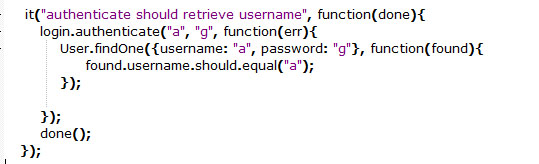
\includegraphics[width=350px]{./TestingDoc/Graphics/usernameTest}
\newline 
\newline 
Code snippets for user login use case, with test data ?g?  . Testing that a valid password is entered
\newline 
\newline
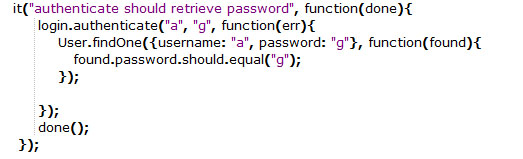
\includegraphics[width=350px]{./TestingDoc/Graphics/passwordTest}
\newline 
\newline
Code snippets for user login use case. Testing that the user is logged in after valid authentication
\newline 
\newline
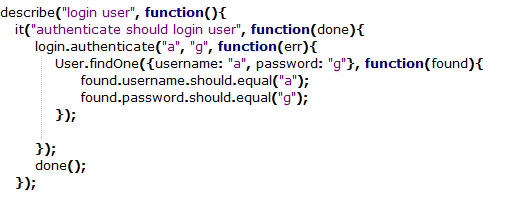
\includegraphics[width=350px]{./TestingDoc/Graphics/UserMustLogIn}

\subsubsection*{Remark}
Login ensures security and access control. Testing regarding the logging in all pass, thus the PIMS system is secure.